\documentclass{beamer}
\usepackage[utf8]{inputenc}
\usepackage{amsmath}
\usepackage{amsfonts}
\usepackage{graphicx}
\usepackage{subcaption}
\usepackage{tikz}
\usetikzlibrary[topaths]
\usepackage{pgfplots}
\setbeameroption{show notes}
\usepackage[sorting=none,backend=bibtex,style=numeric]{biblatex}
\addbibresource{../bibliography/aci-bibliography.bib}
\renewcommand*{\bibfont}{\scriptsize}

\useoutertheme{tree}

\title{Animation character identification from color images}
\author{Alexis Vallet}
\institute{University of Technology of Belfort-Montbéliard}

\begin{document}
\frame{\titlepage}

\section{Animation character identification}

\begin{frame}
\begin{itemize}
\item (Semi) supervised classification of animation character images.
\item Dealing with variations in character posture, occlusion, drawing style, exaggerations.
\item Application domain: web artist communities such as Pixiv, deviantArt.
\end{itemize}

\begin{figure}[htb!]
\centering
\begin{subfigure}{.3\textwidth}

\includegraphics[width=\textwidth]{../images/miku_e.png}
\end{subfigure}
\begin{subfigure}{.3\textwidth}

\includegraphics[width=\textwidth]{../images/miku_c.png}
\end{subfigure}
\begin{subfigure}{.3\textwidth}

\includegraphics[width=\textwidth]{../images/miku_d.png}
\end{subfigure}
\caption{Images illustrating variations for a single character.}
\label{fig:animationImagesVariations}
\end{figure}

\end{frame}

\begin{frame}
\begin{itemize}
\item Preprocessing: removing outlines, switching color space.
\item Segmentation to isolate parts of interest - hair, clothes, face...
\item Classification by comparing segmentation against training set.
\end{itemize}

\begin{figure}[htb!]
\centerline{
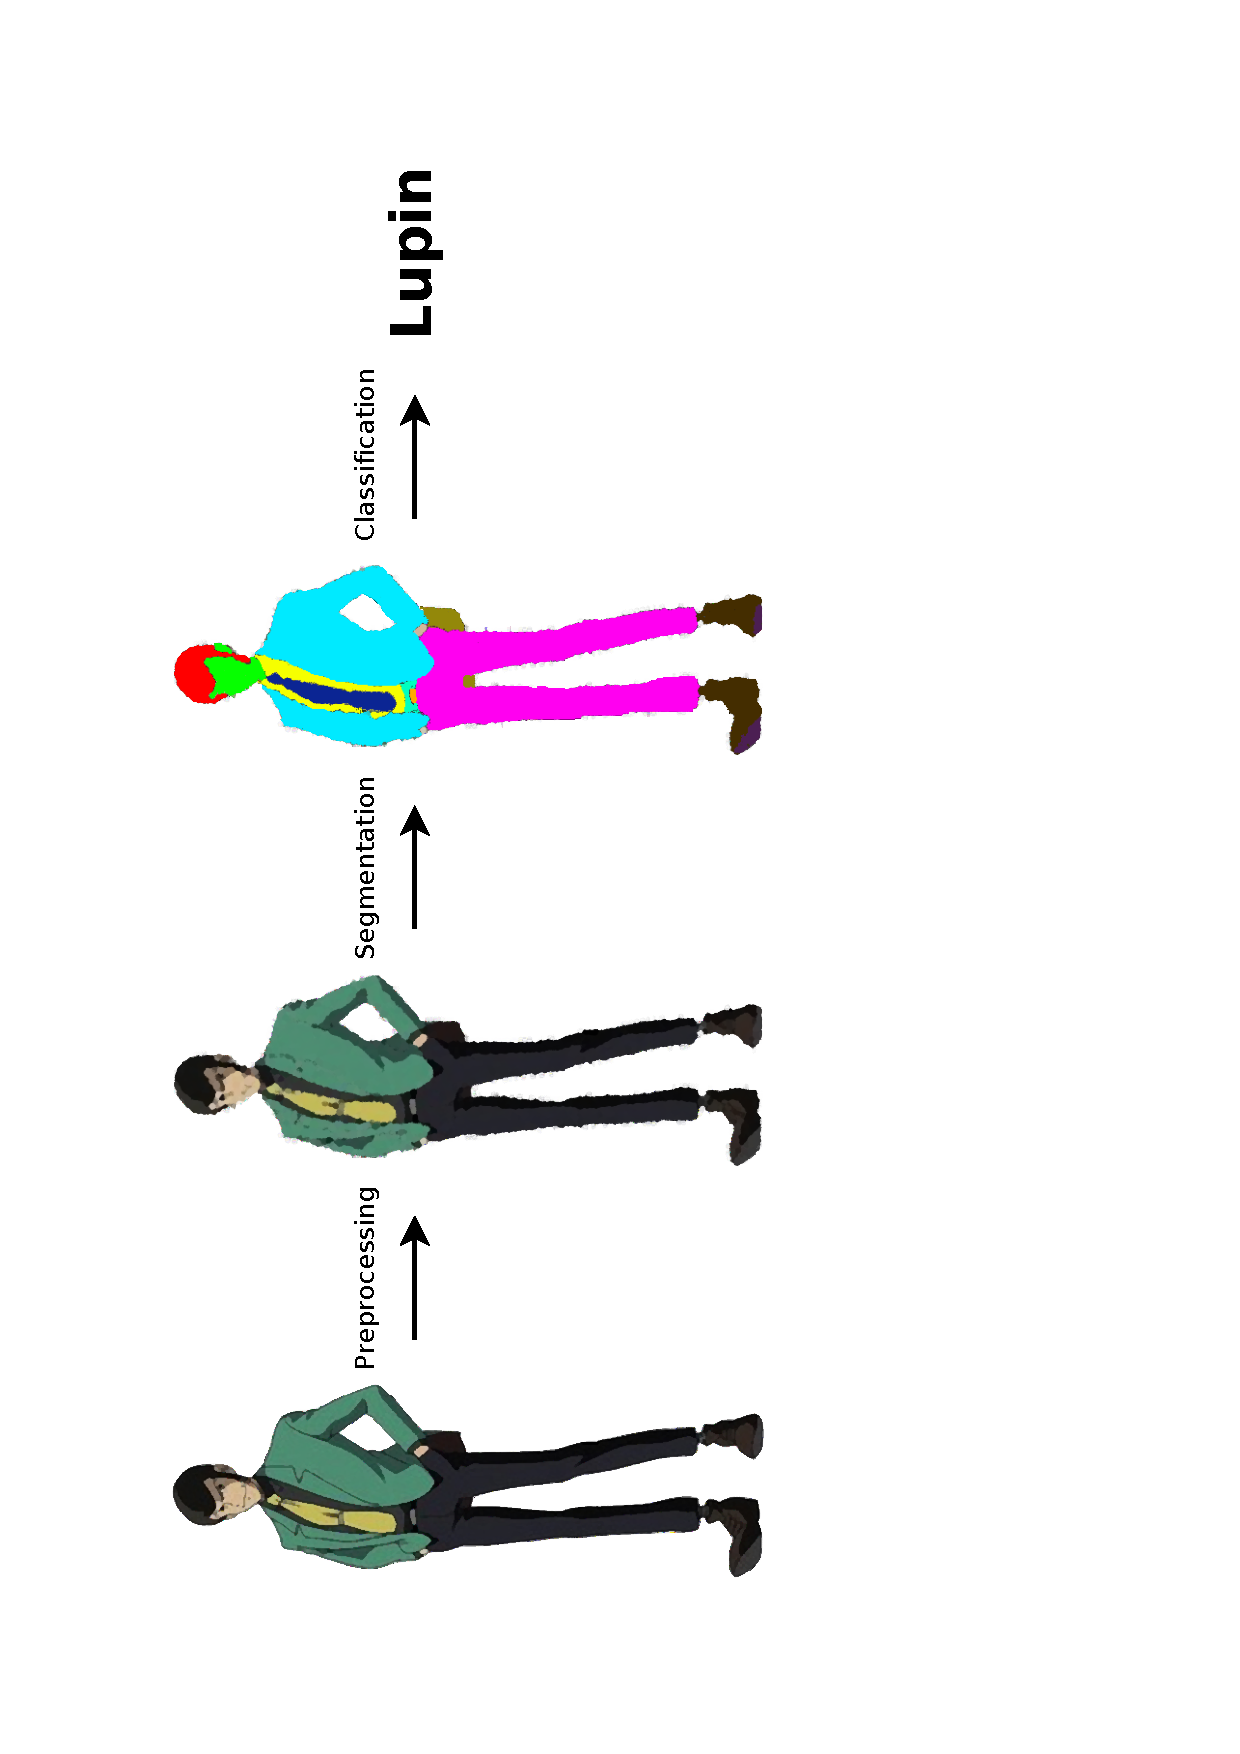
\includegraphics[height=\textwidth,angle=270,clip=true,trim=2cm 0 6cm 0]{../images/visionSystemDiagram.pdf}
}
\caption{Diagram depicting how preprocessing, segmentation and classification interact.}
\end{figure}

\end{frame}

\section{Kuwahara filtering}

\begin{frame}
\begin{itemize}
\item Consider $4$ square windows around the pixel to filter.
\item Compute mean color and variance in lightness (L in HSL) for each window.
\item Assign mean corresponding to smallest variance.
\end{itemize}

\begin{figure}[htb!]
\centering
\begin{subfigure}{.24\textwidth}

\includegraphics[width=\textwidth]{../images/miku_d.png}
\caption{Before filtering.}
\end{subfigure}
\begin{subfigure}{.24\textwidth}

\includegraphics[width=\textwidth]{../images/miku_d_filtered_smallh.png}
\caption{Small window.}
\end{subfigure}
\begin{subfigure}{.24\textwidth}

\includegraphics[width=\textwidth]{../images/miku_d_filtered.png}
\caption{"good" window.}
\end{subfigure}
\begin{subfigure}{.24\textwidth}

\includegraphics[width=\textwidth]{../images/miku_d_filtered_largeh.png}
\caption{Large window.}
\end{subfigure}
\caption{Results of Kuwahara filtering with varying window size.}
\label{fig:kuwaharaExample}
\end{figure}

\end{frame}

\section{Segmentation by Felzenszwalb's method}

\begin{frame}
\frametitle{Felzenszwalb' segmentation \cite{felzenszwalb2004efficient}}

\begin{itemize}
\item Graph method based on Kruskal's algorithm.
\item Efficient: $O(n\log(n))$ time with $4$-connected neighborhood.
\item Accurate: neither too "coarse" nor too "fine".
\item But depends on a scale parameter $k$ which controls the size of segments.
\end{itemize}

\begin{figure}[htb!]
\centering
\begin{subfigure}{.3\textwidth}

\includegraphics[width=\textwidth]{../images/rufy_d.png}
\caption{Original image}
\end{subfigure}
\begin{subfigure}{.3\textwidth}

\includegraphics[width=\textwidth]{../images/luffyK100.png}
\caption{$k = 100$.}
\label{fig:smallKSegmentation}
\end{subfigure}
\begin{subfigure}{.3\textwidth}

\includegraphics[width=\textwidth]{../images/luffyK1000.png}
\caption{$k = 1000$.}
\label{fig:largeKSegmentation}
\end{subfigure}
\end{figure}

\end{frame}

\begin{frame}
\begin{itemize}
\item Compute $4$/$8$-connected graph on the pixels of the image.
\item Edges weighted by euclid distance in color space:
\[
w(u_1, u_2) = ||(l_1,a_1,b_1) - (l_2,a_2,b_2)||
\]
\item Consider edges in ascending weight order.
\item Fuse segments $C_1$, $C_2$ related by edge $(u_1,u_2)$ if $w(u_1,u_2) \leq MInt(C_1, C_2)$.
\end{itemize}

\[
MInt(C_1, C_2) = \min(Int(C_1) + \tau(C_1), Int(C_2) + \tau(C_2))
\]

Where $Int(C) = \max_{\{u,v\} \in MST(C, E)} w(u,v)$, and $\tau(C) = \frac{k}{\sum_{v \in C} d_v}$.

\end{frame}

\begin{frame}
\begin{itemize}
\item Post processing by merging segments with close hue.
\item Allows varying segment sizes and non locally connected segments.
\end{itemize}

\begin{figure}[htb!]
\centering
\begin{subfigure}{0.3\textwidth}

\includegraphics[width=\textwidth]{../images/miku_a.png}
\caption{Original image.}
\end{subfigure}
\begin{subfigure}{0.3\textwidth}
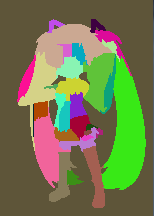
\includegraphics[width=\textwidth]{../images/miku_seg_initial.png}
\caption{Before merging.}
\end{subfigure}
\begin{subfigure}{0.3\textwidth}
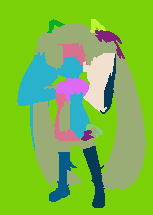
\includegraphics[width=\textwidth]{../images/miku_seg_fused.png}
\caption{After merging.}
\end{subfigure}
\end{figure}
\end{frame}

\section{Classification by spectral method}

\begin{frame}
\frametitle{Spectral classification method}
\begin{itemize}
\item For segmentation $S$ consider features $(f_i : S \rightarrow \mathbb{R}^q_i)_{1 \leq i \leq m}$. (average color, gravity center, size...)
\item For each feature $f_i$, compute $K$-nearest neighbor graph $G_i$ on $S$ with weights $w(u,v) = e^{-\frac{||f_i(S_u) - f_i(S_v)||^2}{\sigma_i^2}}$ and Laplacian $L_i$.
\item Classifying images according to the eigenvectors of the Laplacians.
\end{itemize}

\begin{figure}[htb!]
\centering
\begin{subfigure}{0.3\textwidth}
\centering
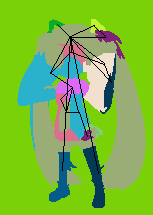
\includegraphics[width=0.7\textwidth]{../images/miku_seg_graph.png}
\caption{Example of graph on $S$.}
\end{subfigure}
\begin{subfigure}{0.65\textwidth}
\resizebox{\hsize}{!}{
$L_i(u,v) = \begin{cases}
\sum_{u'\text{ adjacent to }u} w(u,u') & \text{if } u = v\\
-w(u,v) & \text{if $u$ and $v$ are adjacent}\\
0 & \text{otherwise}
\end{cases}$
}
\caption{Laplacian matrix definition.}
\end{subfigure}
\end{figure}
\end{frame}

\begin{frame}
Method from Wilson, Hancock, Luo \cite{wilson2005pattern}, with some changes:
\begin{itemize}
\item Compute $k$ eigenvectors corresponding to smallest non zero eigenvalues of Laplacian $L_i \in \mathbb{R}^{n \times n}$.
\item Invariance by vertex permutation using symmetric polynomials $P = (P_1, ..., P_n)$.
\item Difference in number of vertices by padding with zeros.
\item Classifying concatenated vectors $E_j$ with SVM.
\end{itemize}

\begin{figure}
\begin{subfigure}{0.49\textwidth}
\resizebox{\hsize}{!}{
$\Phi = (\sqrt{\lambda_1}e_1 ... \sqrt{\lambda_k}e_k) \in \mathbb{R}^{n \times k}$
}
\caption{$e_j$ is eigenvector of $L_i$ corresponding to $\lambda_j$}
\end{subfigure}
\begin{subfigure}{0.49\textwidth}
\resizebox{\hsize}{!}{
$E_j = \begin{pmatrix}
signum(P_1(\Phi_j)) \ln(1 + |P_1(\Phi_j)|) \\
... \\
signum(P_n(\Phi_j)) \ln(1 + |P_n(\Phi_j)|)
\end{pmatrix}$
}
\caption{Where $\Phi_j$ denotes the $j^{th}$ column of $\Phi$}
\end{subfigure}
\end{figure}

\end{frame}

\begin{frame}
\frametitle{Results and analysis}
\begin{itemize}
\item Low recognition rate (close to random).
\item Graphs do not encode enough information about individual segments.
\item Deals poorly with different number of segments.
\item Could be salvaged with dimensionality reduction?
\end{itemize}
\end{frame}

\section{Classification by segment matching}

\begin{frame}
\frametitle{Segment matching classification}
\begin{itemize}
\item Consider $3$ features for each segment: average $L^*a^*b^*$ color, gravity center, and area.
\item Measure similarity between segments using a fuzzy system.
\item Find a one to one relation between similar segments of $2$ images.
\end{itemize}

\begin{figure}
\centering
\begin{subfigure}{0.24\textwidth}

\includegraphics[width=\textwidth]{../images/rufy_d.png}
\end{subfigure}
\begin{subfigure}{0.24\textwidth}
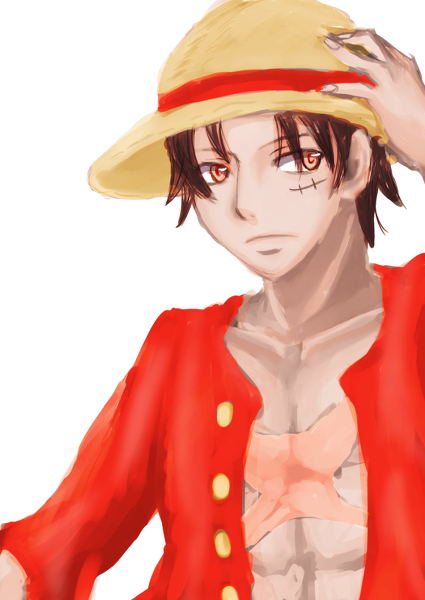
\includegraphics[width=\textwidth]{../images/rufy_original2.png}
\end{subfigure}
\begin{subfigure}{0.24\textwidth}
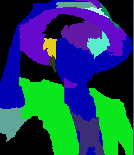
\includegraphics[width=\textwidth]{../images/luffy_match1.png}x
\end{subfigure}
\begin{subfigure}{0.24\textwidth}
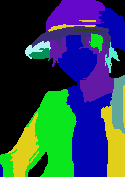
\includegraphics[width=\textwidth]{../images/luffy_match2.png}
\end{subfigure}
\caption{Original images (left) and corresponding relation (right). Segments with the same color are matched together.}
\end{figure}

\end{frame}

\begin{frame}
\begin{figure}[htb!]
\centering
\begin{subfigure}{\textwidth}
\centering
\tikzstyle{block} = [draw, fill=blue!20, rectangle, 
    minimum height=6em, minimum width=6em]
\tikzstyle{pinstyle} = [pin edge={to-,thin,black}]
\begin{tikzpicture}[scale=0.3]
\node (colInput) {$c_{ij} = e^{-\frac{||c_i - c_j||}{\sigma_c^2}}$};
\node [below of=colInput] (posInput) {$x_{ij} = e^{-\frac{||x_i - x_j||}{\sigma_x^2}}$};
\node [below of=posInput] (areaInput) {$a_{ij} = e^{-\frac{|a_i - a_j|}{\sigma_a^2}}$};
\node [block, right of=posInput, node distance=3cm] (fcs) {FCS};
\node [right of=fcs, node distance=3cm] (output) {$s_{ij}$};
\draw [->] (colInput) -- (fcs);
\draw [->] (posInput) -- (fcs);
\draw [->] (areaInput) -- (fcs);
\draw [->] (fcs) -- (output);
\end{tikzpicture}
\caption{Inputs and output.}
\end{subfigure}
\begin{subfigure}{0.33\textwidth}
\centering
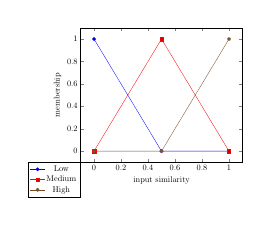
\begin{tikzpicture}[scale=0.3]
\begin{axis}[xlabel=input similarity,ylabel=membership,
legend style={
at={(0,0)},
anchor=north east}]
\addplot coordinates {(0,1) (0.5, 0) (1, 0)};
\addlegendentry{Low}
\addplot coordinates {(0,0) (0.5, 1) (1, 0)};
\addlegendentry{Medium}
\addplot coordinates {(0,0) (0.5,0) (1, 1)};
\addlegendentry{High}
\end{axis}
\end{tikzpicture}
\caption{Inputs membership functions.}
\end{subfigure}
\begin{subfigure}{0.33\textwidth}
\centering
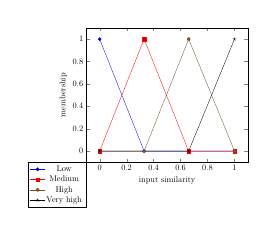
\begin{tikzpicture}[scale=0.3]
\begin{axis}[xlabel=input similarity,ylabel=membership,
legend style={
at={(0,0)},
anchor=north east}]
\addplot coordinates {(0,1) (0.33, 0) (1, 0)};
\addlegendentry{Low}
\addplot coordinates {(0,0) (0.33, 1) (0.66, 0) (1, 0)};
\addlegendentry{Medium}
\addplot coordinates {(0,0) (0.33,0) (0.66, 1) (1, 0)};
\addlegendentry{High}
\addplot coordinates {(0,0) (0.66, 0) (1, 1)};
\addlegendentry{Very high}
\end{axis}
\end{tikzpicture}
\caption{Output membership functions.}
\end{subfigure}
\caption{Segment similarity fuzzy control system.}
\label{fig:segmentFCS}
\end{figure}
\end{frame}

\begin{frame}
\begin{itemize}
\item Measure overall similarity $sim(S,T)$ between segmentation $S$ and $T$ by sum of matching segments similarity weighted by segment areas.
\item Classify by nearest neighbor.
\end{itemize}

\begin{figure}
\centering
\begin{subfigure}{0.3\textwidth}
\centering
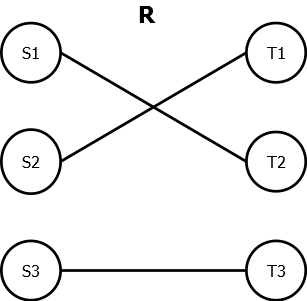
\includegraphics[width=\textwidth]{../images/relation.png}
\end{subfigure}
\begin{subfigure}{0.5\textwidth}
\centering
\[ \quad sim(S,T) = \sum_{(S_i,T_j) \in R}(|S_i| + |T_j|)s_{ij}\]
\end{subfigure}
\end{figure}

Where $s_{ij}$ denotes the similarity between segments $S_i$ and $T_j$ computed by the fuzzy control system.

\end{frame}

\begin{frame}
\frametitle{Results and analysis}
\begin{itemize}
\item $59\%$ recognition rate for dataset with 12 characters and 15 images per character for a total of 180 images.
\item Recognition rate scales well with size of dataset.
\item Has trouble with characters sharing similar color palette.
\end{itemize}

\begin{figure}[htb!]
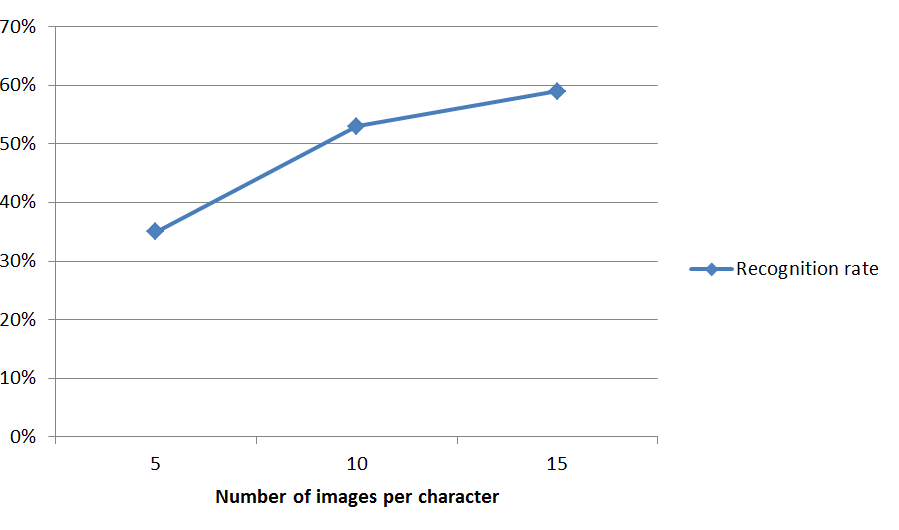
\includegraphics[width=0.8\textwidth]{../images/recognitionRate.png}
\end{figure}

\end{frame}

\begin{frame}
Possible extensions:

\begin{itemize}
\item Color palette issues: determining a (possibly non-linear, or high-dimensional) color space ideally separating training data, with some (semi) supervised embedding method  \cite{urahama2007semi} ?
\item Background extraction: detecting important character features (face, hair, clothes) using method inspired by the face detection algorithm from Viola and Jones \cite{viola2004robust} ?
\item Also using segmentation graph, as in works from Bach and Harchaoui \cite{harchaoui2007image} ?
\end{itemize}
\end{frame}

\section{References}
\begin{frame}
\frametitle{References}
\begin{small}
\printbibliography
\end{small}
\end{frame}

\end{document}